\documentclass[]{article}
\usepackage[T1]{fontenc}
\usepackage[utf8]{inputenc}
%\usepackage[icelandic]{babel}
\usepackage{caption}
\usepackage{circuitikz}
\usepackage{grffile} 
\usepackage[margin=1in]{geometry}

% grffile er pakki sem leifir manni að nota "" til þess að forðast að nota
% nafnið á myndinni með.
\usepackage{graphicx}
% \graphicspath{{images/}} Sýnir undir möppu þar sem myndirnar eru

\usepackage{hyperref}
%fyrirlinka - \url{www.....}
\begin{document}


\title{Formleg mál og reiknanleiki}
\author{Pétur}
\maketitle

\section*{1.}

\subsection*{a)}

\begin{tabular}{ l|l|l }
  String & Machine(a) & Machine(b) \\ \hline
  aaaaa & 	Yes 	& Yes \\
  bbbbb  & 	No	 	& No \\
  abba	&	Yes		& Yes \\
  baba	&	No		& No 
\end{tabular}

\section*{2.}

\begin{tabular}{ll}
a) & Yes \\
b) & Yes \\
c) & Yes 
\end{tabular}

\section*{3.}

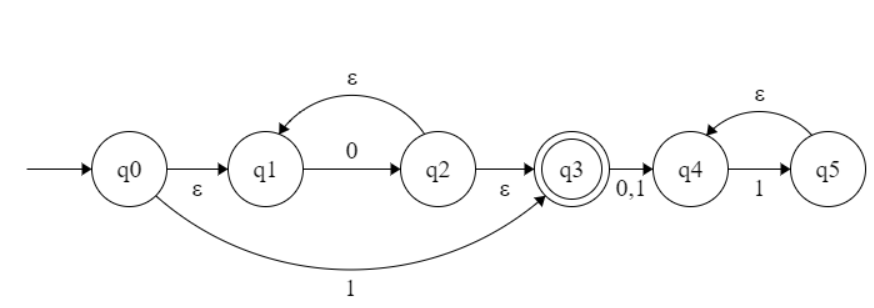
\includegraphics[scale=1]{mynd}

\section*{4.}

\begin{tabular}{l|l|l}
	&	Input	&	Output 	\\ \hline
a)	&	011		&	000 	\\ \hline
b) 	& 	211		&	111 	\\ \hline
c)	&	0202	&	0101	\\
\end{tabular}
\end{document}